% Simple poster (portrait)
% Author: Sofia Jijon (https://sjijon.github.io)
% Last Update: Sept 9, 2021
% Latest Version: https://github.com/sjijon/TeX-templates/tree/main/Tikzposter%20posters/Simple%20poster

\documentclass[a0paper,portrait,margin=0pt, colspace=24pt,subcolspace=0pt,blockverticalspace=36pt,innermargin=50pt]{tikzposter}

\usepackage{amssymb,amsfonts,amsmath,latexsym,amsthm,bm}
%\usepackage[usenames,dvipsnames]{color}
%\usepackage{enumitem}
%\theoremstyle{plain}
\newtheorem{theorem}{Theorem}
%\newtheorem{corollary}[theorem]{Corollary}
%\newtheorem{lemma}[theorem]{Lemma}
%\newtheorem{proposition}[theorem]{Proposition}
%\newtheorem{condition}[theorem]{Condition}
%\newtheorem{algorithm}[theorem]{Algorithm}

\usepackage[latin9]{inputenc}
\usepackage[square,numbers]{natbib} 	% Bibliography manager
\usepackage{amsmath,amssymb}
\usepackage{lipsum}  				    % Random Text
\usepackage[colalign]{aligncolsatbottom}  %To align columns at bottom (!! please run 2 times)
%\newcommand{\bth}{\bm{\theta}}
\newcommand{\la}{\lambda}
\newcommand{\bl}{\bm{\lambda}}
%\newcommand{\bxi}{\bm{\xi}}
\newcommand{\bsee}{\bm{\Sigma_e}}
\newcommand{\bo}{\bm{\Omega}}
\newcommand{\bD}{\bm{\Delta}}
%\newcommand{\bse}{\bm{\Sigma_e}^{-1}}
\newcommand{\bT}{\bm{t}}
%\newcommand{\bh}{\bm{H}}
\newcommand{\bc}{\bm{C}}
%\newcommand{\bd}{\bm{D}}
\newcommand{\bww}{\bm{W}}
%\newcommand{\ba}{\bm{A}}
\newcommand{\bbb}{\bm{B}}
\newcommand{\bg}{\bm{G}}
\newcommand{\bmy}{\bm{y}}
%\newcommand{\bys}{\bm{y^*}}
\newcommand{\bdd}{\bm{\delta}}
\newcommand{\bdh}{\hat{\bm{\delta}}}
%\newcommand{\byst}{\bm{y^{*T}}}

\newcommand{\thatb}{\hat{\bm{\theta}}^B}
\newcommand{\thatt}{\hat{\bm{\theta}}}
\newcommand{\thattt}{\hat{\bm{\theta_2}}}
\newcommand{\thp}{\hat{\bm{\theta}}^p}
\newcommand{\thg}{\hat{\bm{\theta}}^g}
\newcommand{\thbm}{\hat{\bm{\theta}}^{BM}}

\newcommand{\bty}{\tilde{\bm{\theta}}_{y,t}}
\newcommand{\su}{{\sigma_u^2}}
\newcommand{\thh}{{\theta}}
\newcommand{\bgam}{\bm{\gamma}}
\newcommand{\bth}{\bm{\theta}}
\newcommand{\bxi}{\bm{x}_i}
\newcommand{\bse}{\bm{\Sigma_e}^{-1}}
\newcommand{\bh}{\bm{H}}
\newcommand{\bd}{\bm{D}}
%\newcommand{\ba}{\bm{A}}
\newcommand{\bb}{\bm{\beta}}
% y\newcommand{\bxi}{\bm{x}_i}
\newcommand{\bys}{\bm{y^*}}
\newcommand{\byst}{\bm{y^{*T}}}
\newcommand{\V}       {\text{Var}}
\newcommand{\de}       {\mbox{$\delta_i$}}
\newcommand{\tij}       {\mbox{$\theta_{ij}$}}
\newcommand{\htijb}       {\mbox{$\hat{\theta}_{ij}^B$}}

\newcommand{\thbariw}     {\mbox{$\bar{\hat{\theta}}_{iw}^{B}$}}
\newcommand{\tbw}       {\mbox{$\bar{\theta}_{w}^B$}}
\newcommand{\tbiw}       {\mbox{$\bar{\theta}_{iw}$}}
\newcommand{\thwb}       {\mbox{$\bar{\hat\bm{{\theta}}}_{w}^B$}}
\newcommand{\thw}       {\mbox{$\bar{\hat{\theta}}_{w}^B$}}
\newcommand{\thbiw}       {\mbox{$\bar{\hat{\theta}}_{iw}^B$}}
\newcommand{\that}       {\mbox{$\hat{\theta}$}}
\newcommand{\thij}       {\mbox{$\hat{\theta}_{ij}$}}
\newcommand{\thhi}       {\mbox{$\hat{\theta}_{i}$}}
\newcommand{\thi}       {\theta_i}

%\newcommand{\lt}       {\left}
%\newcommand{\rt}       {\right}
\newcommand{\lao}       {\mbox{$\lambda_{1i}$}}
\newcommand{\lat}       {\mbox{$\lambda_{2}$}}
\newcommand{\latt}       {\mbox{$\lambda_{3i}$}}


\newcommand{\cd}{\buildrel d \over \longrightarrow}
\newcommand{\cp}{\buildrel P \over \longrightarrow}
%\newcommand{\R}{\mathbb{R}}
\newcommand{\hatbb}{\boldsymbol{\hat{b}}}
\newcommand{\hatbB}{\boldsymbol{\hat{B}}}
\newcommand{\hatbd}{\boldsymbol{\hat{d}}}
\newcommand{\commentt}[1]{}
\newcommand{\myvfil}[1]{\vskip 0pt plus #1fill}
% \renewcommand{\upsilon}{v}
\newcommand{\lik}{\ell_y(\theta)}
\newcommand{\likil}{\ell_y(\theta_i^{(l)})}
\newcommand{\hd}{\hfill$\diamondsuit$}
\newcommand{\aaa}{\epsilon}
\newcommand{\lt}{\left}
\newcommand{\rt}{\right}
\newcommand{\mbi}{\max_{1 \leq i \leq m} \bxi'\bb}
\newcommand{\bs}{B_{i*}}
\newcommand{\D}{\Delta}
\newcommand{\bi}{B_{i}}
%\newcommand{\that}        {\mbox{$\hat{\boldsymbol{\theta}}$}}
\newcommand{\utheta}        {\mbox{$\boldsymbol{\theta}$}}
\newcommand{\thhj}{\hat{\theta}_j}
\newcommand{\thhij}{\hat{\theta}_{ij}}
\newcommand{\thiHB}{\hat{\theta}_i^{HB}}
\newcommand{\thih}{\hat{\theta}_i^H}
\newcommand{\thit}{\tilde{\theta}_i^H}
%\newcommand{\V}{\text{Var}}

\newcommand{\tr}{\text{tr}}
\newcommand{\btt}{\boldsymbol{\theta}}

\newcommand{\ttt}{\boldsymbol{t}}
\newcommand{\bhat}{\boldsymbol{\hat{\beta}}}
\newcommand{\thb}{\bar{\theta}}
\newcommand{\bx}{\bm{x}}
\newcommand{\bX}{\bm{X}}
\newcommand{\bY}{\boldsymbol{Y}}
\newcommand{\lam}{\boldsymbol{\Lambda}}
\newcommand{\pxv}{{P}_X^V}
\newcommand{\pxvt}{\bar{P}_x^{V'}}
\newcommand{\pxvs}{\bar{P}_x^{V_*}}
\newcommand{\bv}{\boldsymbol{v}}
\newcommand{\bu}{\boldsymbol{u}}
\newcommand{\ur}{\boldsymbol{r}}
\newcommand{\uphi}{\boldsymbol{\phi}}
\newcommand{\uone}{\boldsymbol{1}}
\newcommand{\ue}{\boldsymbol{e}}
\newcommand{\uc}{\boldsymbol{c}}
\newcommand{\bbi}{\boldsymbol{b}_i}
\newcommand{\uw}{\boldsymbol{w}}
\newcommand{\bz}{\boldsymbol{z}}
\newcommand{\be}{\boldsymbol{e}}
\newcommand{\by}{\boldsymbol{y}}
\newcommand{\utt}{\boldsymbol{t}}
\newcommand{\bzero}{\boldsymbol{0}}
%\newcommand{\bl}{\boldsymbol{l}}
\newcommand{\util}{\boldsymbol{\tilde{u}}}
\newcommand{\utils}{\boldsymbol{\tilde{u}_*}}
\newcommand{\btil}{\boldsymbol{\tilde{\beta}}}
\newcommand{\btils}{\boldsymbol{\tilde{\beta}^{*}}}
%\newcommand{\bm}{\boldsymbol{m}}
\newcommand{\btilf}{(X'V^{-1}X)^{-1}X'V^{-1}\that}
\newcommand{\btilfs}{(X'V_*^{-1}X)^{-1}X'V_*^{-1}\that}
\newcommand{\bxij}{\boldsymbol{x_{ij}}}
\newcommand{\bxj}{\boldsymbol{x_{j}}}
\newcommand{\bei}{\boldsymbol{e_{i}}}
\newcommand{\bej}{\boldsymbol{e_{j}}}
\newcommand{\bek}{\boldsymbol{e_{k}}}
\newcommand{\bbary}{\boldsymbol{\bar{y}}}
\newcommand{\thet}{\boldsymbol{\theta}}



%\newcommand{\lao}       {\mbox{$\lambda_{1i}$}}
%\newcommand{\lat}       {\mbox{$\lambda_{2}$}}
%\newcommand{\latt}       {\mbox{$\lambda_{3i}$}}


\newcommand{\vv}        {V^{-1}}
\newcommand{\vs}        {V^{-1}_*}
\newcommand{\vvs}        {V_{*}}
\newcommand{\sig}        {\Sigma}
\newcommand{\sm}        {\sqrt{m}}
%\newcommand{\thi}        {\theta_i}
%\newcommand{\thhi}        {\mbox{$\hat{\theta}_i$}}
\newcommand{\thhk}        {\mbox{$\hat{\theta}_k$}}
\newcommand{\thho}        {\mbox{$\hat{\theta}_1$}}
\newcommand{\thhm}        {\mbox{$\hat{\theta}_m$}}
\newcommand{\thj}        {\mbox{$\hat{\theta}_j$}}
%\newcommand{\thij}        {\mbox{$\hat{\theta}_{ij}$}}
\newcommand{\ttil}        {\mbox{$\tilde{\boldsymbol{\theta}}$}}

\newcommand{\thk}        {\mbox{$\hat{\theta}_k$}}
%\newcommand{\tij}       {\mbox{$\theta_{ij}$}}
\newcommand{\thbi}        {\mbox{$\hat{\theta}_i^B$}}
\newcommand{\thbis}        {\mbox{$\hat{\theta}_{i*}^B$}}
\newcommand{\thebis}        {\mbox{$\hat{\theta}_{i*}^{EB}$}}
\newcommand{\thebjs}        {\mbox{$\hat{\theta}_{j*}^{EB}$}}
\newcommand{\thbj}        {\mbox{$\hat{\theta}_j^B$}}
\newcommand{\thbjs}        {\mbox{$\hat{\theta}_{j*}^B$}}
\newcommand{\thbk}        {\mbox{$\hat{\theta}_k^B$}}
%\newcommand{\htijb}        {\mbox{$\hat{\theta}_{ij}^B$}}
\newcommand{\thebi}       {\mbox{$\hat{\theta}_i^{EB}$}}
\newcommand{\thebj}       {\mbox{$\hat{\theta}_j^{EB}$}}
\newcommand{\theblupi}    {\mbox{$\hat{\theta}_i^{EBM1}$}}
\newcommand{\thbmi}    {\mbox{$\hat{\theta}_i^{BM1}$}}
\newcommand{\theblupis}       {\mbox{$\hat{\theta}_{i*}^{EBM1}$}}

%\newcommand{\thbiw}       {\mbox{$\bar{\hat{\theta}}_{iw}^B$}}
\newcommand{\thhw}       {\mbox{$\bar{\hat{\theta}}_{w}$}}
%\newcommand{\thw}       {\mbox{$\bar{\hat{\theta}}_{w}^B$}}
%\newcommand{\tbiw}       {\mbox{$\bar{\theta}_{iw}$}}
%\newcommand{\thbariw}     {\mbox{$\bar{\hat{\theta}}_{iw}^{B}$}}
\newcommand{\thbarw}     {\mbox{$\bar{\hat{\theta}}_{w}^{B}$}}
\newcommand{\thbarwb}     {\mbox{$\bar{\hat{\theta}}_w^{B}$}}
\newcommand{\thbarwbs}     {\mbox{$\bar{\hat{\theta}}_{w*}^{B}$}}
\newcommand{\thbarweb}     {\mbox{$\bar{\hat{\theta}}_w^{EB}$}}
\newcommand{\thbarwebs}     {\mbox{$\bar{\hat{\theta}}_{w*}^{EB}$}}
%\newcommand{\se}     {\mbox{$\sigma_{ei}^2$}}
%\newcommand{\su}    {\sigma_u^2}
\newcommand{\sbb}     {\mbox{$\sigma_b^2$}}
\newcommand{\sut}     {\mbox{$\tilde{\sigma}_u^2$}}
\newcommand{\suh}     {\mbox{$\hat{\sigma}_u^2$}}
\newcommand{\sus}     {\mbox{${\sigma}_u^{*2}$}}
\newcommand{\sust}     {\mbox{$\tilde{\sigma}_u^{*2}$}}
%\newcommand{\btil}     {\mbox{$(X'V^{-1}X)^{-1}X'V^{-1}\boldface{\theta}$}}
\newcommand{\hvis}     {\mbox{$\boldsymbol{x}_i'(X'V^{-1}_*X)^{-1}\boldsymbol{x}_i$}}
\newcommand{\hvi}     {\mbox{$\boldsymbol{x}_i'(X'V^{-1}X)^{-1}\boldsymbol{x}_i$}}
\newcommand{\hij}     {\mbox{$\boldsymbol{x}_i'(X'X)^{-1}\boldsymbol{x}_j$}}
\newcommand{\hvk}     {\mbox{$\boldsymbol{x}_k'(X'V^{-1}X)^{-1}\boldsymbol{x}_k$}}
\newcommand{\hj}     {\max_{1\leq j \leq m} h_j}
\newcommand{\hi}     {\max_{1\leq i \leq m} h_i}
\newcommand{\hk}     {\mbox{$\boldsymbol{x}_k'(X'X)^{-1}\boldsymbol{x}_k$}}
\newcommand{\hvik}     {\mbox{$\boldsymbol{x}_i'(X'V^{-1}X)^{-1}\boldsymbol{x}_k$}}
\newcommand{\hii}     {\mbox{$\boldsymbol{x}_i'(X'X)^{-1}\boldsymbol{x}_i$}}
%\newcommand{\bt}     {\mbox{$\tilde{\bm{\beta}}$}}
\newcommand{\ut}     {\mbox{$\tilde{\boldsymbol{u}}$}}
\newcommand{\uts}     {\mbox{$\tilde{\boldsymbol{u}}_*$}}
\newcommand{\ub}     {\mbox{${\boldsymbol{u}}$}}
%\newcommand{\bb}     {\mbox{${\boldsymbol{\beta}}$}}
\newcommand{\li}     {\mbox{${\lambda_i}$}}
\newcommand{\lj}     {\mbox{${\lambda_j}$}}
\newcommand{\lk}     {\mbox{${\lambda_k}$}} 
\newcommand{\co}     {\text{Cov}}
\newcommand{\lp}     {\left(}
\newcommand{\rp}     {\right)}
\newcommand{\lb}     {\left[}
\newcommand{\rb}     {\right]}
\newcommand{\gos}     {G_1^{*}}
\newcommand{\gtos}     {G_2^{*}}
\newcommand{\gts}     {G_3^{*}}
%\newcommand{\g}     {\mbox{$X(X'V^{-1}X)^{-1}X'$}}
\newcommand{\xg}     {\mbox{$(X'V^{-1}X)^{-1}X'$}}
%\newcommand{\bxi}{\boldsymbol{x}_i}
\newcommand{\bw}{\boldsymbol{w}}
\newcommand{\bci}{\boldsymbol{c}_i}
\newcommand{\bgi}{\boldsymbol{g}_i}
\newcommand{\bxk}{\boldsymbol{x}_k}
\newcommand{\byi}{\boldsymbol{y}_i}
\newcommand{\bzi}{\boldsymbol{z}_i}
\newcommand{\bt}{\boldsymbol{\tilde{\beta}}}
\newcommand{\lai}     {\lambda_i}
\newcommand{\gai}     {\gamma_i}
\newcommand{\ma}     {\max_{1 \leq i \leq m}}
\newcommand{\mak}     {\max_{1 \leq k \leq m}}

\newcommand{\cov}     {\text{Cov}}

%%leila/aa commands


\newcommand{\zv}{{\bf z}_v}
\newcommand{\ua}{{\bf u}_a}
\newcommand{\uav}{{\bf u}_{A(v)}}
\newcommand{\sa}{\alpha^2_a}
\newcommand{\bet}{\boldsymbol\beta_v}
\newcommand{\sv}{\nu^2_v}
\newcommand{\se}{\sigma^2_v}
\newcommand{\R}{\mathbb{R}}
\newcommand{\bmu}{\boldsymbol\mu}
\newcommand{\bSigma}{\boldsymbol\Sigma}

% Fix spacing issues with \left and \right
\let\originalleft\left
\let\originalright\right
\renewcommand{\left}{\mathopen{}\mathclose\bgroup\originalleft}
\renewcommand{\right}{\aftergroup\egroup\originalright}

\newcommand{\Prob}{\mathbb{P}}
\newcommand{\Exp}{\mathbb{E}}
\newcommand{\Fe}{\mathscr{F}}
\newcommand{\Borel}{\mathscr{B}}
%\newcommand{\R}{\mathbb{R}}
\newcommand{\N}{\mathbb{N}}
\newcommand{\Rd}{\mathbb{R}^{d}}
\newcommand{\Rplus}{\mathbb{R}_{+}}
%\newcommand{\cntblunion}{\bigcup_{i=1}^{\infty}}
%\newcommand{\cntblinter}{\bigcap_{i=1}^{\infty}}
%\newcommand{\cntblsum}{\sum_{i=1}^{\infty}}

\newcommand{\pd}[2]{\frac{\partial #1}{\partial #2}}
\newcommand{\der}[2]{\frac{d #1}{d #2}}
%\newcommand{\ind}[1]{{\boldsymbol{1}}_{#1}}
\newcommand{\jacobian}[3] {\begin{matrix}
					\pd{#1_{1}}{#2_{1}} & \dots & \pd{#1_{1}}{#2_{#3}}\\
					\vdots & \vdots \\
					\pd{#1_{#3}}{#2_{1}} & \dots & \pd{#1_{#3}}{#2_{#3}}
				\end{matrix}}
%\newcommand{\lam}{\mathbf{\Lambda}}				
\newcommand{\Abs}[1]{\left| #1 \right|}
\newcommand{\vx}{\mathbf{x}}
\newcommand{\vX}{\mathbf{X}}
\newcommand{\ds}[4]{#1_{#2}#4\ldots #4 #1_{#3}}
\newcommand{\vW} {\mathbf{W}}
\newcommand{\vA} {\mathbf{A}}
\newcommand{\vB} {\mathbf{B}}
\newcommand{\vZ} {\mathbf{Z}}
\newcommand{\vY} {\mathbf{Y}}
\newcommand{\vN} {\mathbf{N}}
\newcommand{\vt} {\mathbf{t}}
\newcommand{\vmu} {\mathbf{\mu}}
\newcommand{\vga} {\mathbf{\gamma}}
\newcommand{\vone} {\boldsymbol{1}}
\newcommand{\Xbar} {\overline{X}}
%\newcommand{\C}{\mathbb{C}}
\newcommand{\Sp}{\mathbb{S}}

%
%\newcommand{\freccia}{$\blacktriangleright$}
%\newcommand{\ol}{\overline}
%\newcommand{\ul}{\underline}
%\renewcommand{\baselinestretch}{1.3}
%\newcommand{\expect}{\rm I\hspace{-.25em}E}
%\newcommand{\bpf}{{\bf Proof. }}
%\newcommand{\epf}{\vrule height10pt width5pt depth0pt}
%\newcommand{\bea}{\begin{eqnarray*}}
%\newcommand{\eea}{\end{eqnarray*}}
%\newcommand{\bean}{\begin{eqnarray}}
%\newcommand{\eean}{\end{eqnarray}}
%\newcommand{\bdm}{\begin{displaymath}}
%\newcommand{\edm}{\end{displaymath}}
%\newcommand{\nc}{\nonumber\\}
\def\ie{\emph{i.e.\/}}
\def\eg{\emph{e.g.\/}}
\def\xZ{{\cal Z}}
\def\xA{{\cal A}}
\def\R{\mathbb{R}}
\def\I{1\!{\rm I}}             % indicatrice
\def\ln{\ell_{n}}              % log-vraisemblance
\def\lns{\ell_{n}^{\star}}     % log-vraisemblance
\def\Ti{\Theta^{\infty}}       % Theta infini
\def\T#1{\Theta_{#1}}          % Theta #1
\def\p#1{\pi_{#1}}             % a priori pi #1
\def\ft{f_{\theta}}            % densite
\def\fs{f^{\star}}             % densite
\def\lt{\ell_{\theta}}         % log-densite
\def\ls{\ell^{\star}}          % log-densite
\def\Pt{P_{\theta}}            % proba
\def\Ps{P^{\star}}             % P etoile
\def\Kn{\widehat{K_{n}}}       % estimateur
\def\Ks{K^{\star}}             % K etoile
\def\Es{\mathrm{E}^{\star}}    % E etoile
\def\Et{\mathrm{E}_{\theta}}   % E theta
\def\Etp{\mathrm{E}_{\theta'}}   % E theta prime
\def\Dt{\Delta(\theta)}        % Delta theta
\def\Xn{(X_1, \cdots, X_n)}        % X^n = (X_1,...,X_n)
\def\cm{\left ( X_n; n\geq 0\right )}
\def\xn{(x_1, \cdots, x_n)}        % 

\newcommand\independent{\protect\mathpalette{\protect\independenT}{\perp}}
\def\independenT#1#2{\mathrel{\rlap{$#1#2$}\mkern2mu{#1#2}}}
\def\boldfacefake #1{%
        \hbox{%
                \mathsurround=0pt
                \hbox to 0.25pt{$#1$\hss}%
                \hbox to 0.25pt{$#1$\hss}%
                \hbox {$#1$}%
        }%
}
\newenvironment{mybox}%
{\hspace{-0.15 cm}
\begin{Sbox}
\begin{minipage}{12 cm}
 \vspace{0.15 cm} }%
{\vspace{0.15 cm} 
\end{minipage}
\end{Sbox}
\fbox{\TheSbox}}

\def\bfalpha{\mbox{$\boldfacefake{\alpha}$}}
\def\bftheta{\mbox{$\boldfacefake{\theta}$}}
\def\bflambda{\mbox{$\boldfacefake{\lambda}$}}
\def\bfmu{\mbox{$\boldfacefake{\mu}$}}
\def\bfnu{\mbox{$\boldfacefake{\nu}$}}
\def\bfpsi{\mbox{$\boldfacefake{\psi}$}}
\def\bfxi{\mbox{$\boldfacefake{\xi}$}}
\def\bfepsilon{\mbox{$\boldfacefake{\epsilon}$}}
\def\bfPsi{\mbox{$\boldfacefake{\Psi}$}}
\def\bfTheta{\mbox{$\boldfacefake{\Theta}$}}

\def\bfh{\mbox{$\boldfacefake{h}$}}
\def\bfb{\mbox{$\boldfacefake{b}$}}
\def\bfl{\mbox{$\boldfacefake{l}$}}
\def\bfm{\mbox{$\boldfacefake{m}$}}
\def\bfp{\mbox{$\boldfacefake{p}$}}
\def\bfu{\mbox{$\boldfacefake{u}$}}
\def\bfy{\mbox{$\boldfacefake{y}$}}
\def\bfA{\mbox{$\boldfacefake{A}$}}
\def\bfB{\mbox{$\boldfacefake{B}$}}
\def\bfC{\mbox{$\boldfacefake{C}$}}
\def\bfD{\mbox{$\boldfacefake{D}$}}
\def\bfH{\mbox{$\boldfacefake{H}$}}
\def\bfI{\mbox{$\boldfacefake{I}$}}
\def\bfP{\mbox{$\boldfacefake{P}$}}
\def\bfR{\mbox{$\boldfacefake{R}$}}
\def\bfS{\mbox{$\boldfacefake{S}$}}

%%% probability symbolism
\newcommand{\proba}{\operatorname{Pr}}
\newcommand{\esl}{\end{slide}}
\newcommand{\bsl}{\begin{slide}}
\newcommand{\ok}{\blacksquare}

\newcommand{\prob}[1]{\operatorname{Pr}\left( #1 \right)}
\newcommand{\hprob}[1]{\hat{Pr}\left( #1 \right)}
\newcommand{\probpi}[1]{\operatorname{Pr}^{\pi}(#1)}
\newcommand{\probte}[1]{\operatorname{Pr}_{\te}(#1)}
\newcommand{\probstar}[1]{\operatorname{Pr}^*(#1)}
\newcommand{\expi}[1]{\operatorname{I\hspace{-.25em}E^{\pi}}\left(#1\right)}
\newcommand{\exy}[1]{\operatorname{I\hspace{-.25em}E_{Y}}\left(#1\right)}
\newcommand{\exmu}[1]{\operatorname{I\hspace{-.25em}E^{\mu}}\left(#1\right)}
\newcommand{\extet}[1]{\operatorname{I\hspace{-.25em}E_{\theta}}\left(#1\right)}
\newcommand{\vartet}[1]{\operatorname{Var_{\theta}}\left(#1\right)}
\newcommand{\extez}[1]{\operatorname{I\hspace{-.25em}E_{\theta_0}}\left(#1\right)}
\newcommand{\expom}[1]{\operatorname{I\hspace{-.25em}E_{\omega}}\left(#1\right)}
\newcommand{\expectsub}[2]{\operatorname{I\hspace{-.25em}E_{#1}}\left[#2\right]}
\newcommand{\expectsugiu}[3]{{\operatorname{I\hspace{-.25em}E}_{#1}^{#2}}\left[#3\right]}
\newcommand{\expectup}[2]{\operatorname{I\hspace{-.25em}E^{#1}}\left[#2\right ]}
\newcommand{\bxii}{\bx_{(-i)}}
\newcommand{\expe}[1]{\operatorname{\rm I\hspace{-.25em}E}\left(#1\right)}
\newcommand{\diag}[1]{\operatorname{\rm diag}\left(#1\right)}
\newcommand{\expeq}[1]{\operatorname{\rm I\hspace{-.25em}E}\left [#1\right]}
\newcommand{\rea}{\operatorname{\rm I\hspace{-.25em}R}}
\newcommand{\expeb}[1]{\operatorname{\rm I\hspace{-.25em}E}#1}
%\newcommand{\expeb}[1]{\operatorname{E $#1$}}
\newcommand{\expebb}[2]{\operatorname{\rm I\hspace{-.25em}E}\left(#1\right)^#2}
\newcommand{\bsigma}{\text{\mathversion{bold}$\sigma$\mathversion{normal}}}
\newcommand{\normaldensity}[3] {\frac1{\sqrt{2\pi#3}}\exp\left[-\frac1{2#3} (#1-#2)^2\right]}
\newcommand{\trace}[1]{\operatorname{traccia}\left(#1\right)}
%\newcommand{\tr}[1]{\operatorname{tr}\left(#1\right)}
\newcommand{\etr}[1]{\operatorname{etr}\left(#1\right)}
%%% different fields in mathematics
\newcommand{\integers}{\mathbb{N}}
\newcommand{\itemr}{\item[${\red \bullet}$]}
\newcommand{\reals}{\mathbb{R}}
\newcommand{\Ec}{\`{E}\,\,}
\newcommand{\argmax}{\mbox{\,argmax\,}}
%\newcommand{\argmin}{\mbox{\,argmin\,}}
\newcommand{\iid}{\stackrel{\texttt{iid}}{\sim}}
\newcommand{\ind}{\stackrel{\texttt{ind}}{\sim}}
\newcommand{\indic}[1]{{\boldsymbol{1}}_{#1}}
\newcommand{\posreals}{\reals^+}
\newcommand{\realvectors}[1]{\reals^{#1}}
\newcommand{\complex}{\mathbf{C}}
\newcommand{\ox}{\overline{X}\ }
\newcommand{\id}{\mathbf{id}}
%%% boldface symbolism for multivariate stuff
%%% latin
%\newcommand{\bx}{\mathbf{x}}
%\newcommand{\bX}{\mathbf{X}}
%\newcommand{\bg}{\mathbf{g}}
%\newcommand{\bfG}{\mathbf{G}}
%\newcommand{\bG}{\mathbf{G}}
%\newcommand{\by}{\mathbf{y}}
%\newcommand{\hby}{\hat{\mathbf{y}}}
%\newcommand{\bY}{\mathbf{Y}}
%\newcommand{\bV}{\mathbf{V}}
%\newcommand{\bv}{\mathbf{v}}
%\newcommand{\br}{\mathbf{r}}
%\newcommand{\bR}{\mathbf{R}}
%\newcommand{\bZ}{\mathbf{Z}}
%\newcommand{\bz}{\mathbf{z}}
%\newcommand{\bs}{\mathbf{s}}
%\newcommand{\erre}{{\ttfamily{{\bf R}\,}}}
%\newcommand{\bt}{\mathbf{t}}
%\newcommand{\bT}{\mathbf{T}}
%\newcommand{\bU}{\mathbf{U}}
%\newcommand{\bA}{\mathbf{A}}
%\newcommand{\ba}{\mathbf{a}}
%\newcommand{\be}{\mathbf{e}}
%\newcommand{\bb}{\mathbf{b}}
%\newcommand{\bB}{\mathbf{B}}%
%\newcommand{\bF}{\mathbf{F}}
%\newcommand{\bH}{\mathbf{H}}
%\newcommand{\bQ}{\mathbf{Q}}
%\newcommand{\bc}{\mathbf{c}}
%%\newcommand{\cab}{C_{ab}}
%\newcommand{\gab}{g_{ab}}
%\newcommand{\bC}{\mathbf{C}}
%\newcommand{\bd}{\mathbf{d}}
%%\newcommand{\bs}{\mathbf{s}}
%\newcommand{\bw}{\mathbf{w}}
%\newcommand{\hgz}{\hat{\gamma}_0}
%\newcommand{\hgu}{\hat{\gamma}_1}
%\newcommand{\hp}{\hat{p}}
%\newcommand{\hbe}{\hat{\beta}}
%\newcommand{\hbbe}{\hat{\bbeta}}
%\newcommand{\hte}{\hat{\theta}}
%\newcommand{\bi}{\mathbf{i}}
%\newcommand{\bu}{\mathbf{u}}
%%\newcommand{\bm}{\mathbf{m}}
%\newcommand{\bD}{\mathbf{D}}
%\newcommand{\beffe}{\mathbf{f}}
%\newcommand{\bI}{\mathbf{I}}
%\newcommand{\bM}{\mathbf{M}}
%\newcommand{\bP}{\mathbf{P}}
%\newcommand{\np}{\newpage}
%\newcommand{\bp}{\mathbf{p}}
%\newcommand{\bS}{\mathbf{S}}
%\newcommand{\bJ}{\mathbf{J}}
%\newcommand{\bW}{\mathbf{W}}
%\newcommand{\bzero}
%{\text{\mathversion{bold}$0$\mathversion{normal}}}
%\newcommand{\buno}{
%\text{\mathversion{bold}$1$\mathversion{normal}}}
%%%% and greek
%\newcommand{\bSigma}
%{\text{\mathversion{bold}$\Sigma$\mathversion{normal}}}
%\newcommand{\bmu}{\text{\mathversion{bold}$\mu$\mathversion{normal}}}
%\newcommand{\bpi}{\text{\mathversion{bold}$\pi$\mathversion{normal}}}
%\newcommand{\bnu}{\text{\mathversion{bold}$\nu$\mathversion{normal}}}
%\newcommand{\btheta}{\text{\mathversion{bold}$\theta$\mathversion{normal}}}
%%\newcommand{\erre}{\texttt{{\bf R\,\,}}}
%\newcommand{\bphi}{\text{\mathversion{bold}$\phi$\mathversion{normal}}}
%\newcommand{\bpsi}{\text{\mathversion{bold}$\psi$\mathversion{normal}}}
%\newcommand{\bPsi}{\text{\mathversion{bold}$\Psi$\mathversion{normal}}}
%\newcommand{\bxi}{\text{\mathversion{bold}$\xi$\mathversion{normal}}}
%\newcommand{\balpha}{\text{\mathversion{bold}$\alpha$\mathversion{normal}}}
%\newcommand{\bbeta}{\text{\mathversion{bold}$\beta$\mathversion{normal}}}
%\newcommand{\bdelta}{\text{\mathversion{bold}$\delta$\mathversion{normal}}}
%\newcommand{\boeta}{\text{\mathversion{bold}$\eta$\mathversion{normal}}}
%\newcommand{\bGamma}{\text{\mathversion{bold}$\Gamma$\mathversion{normal}}}
%\newcommand{\bve}{\text{\mathversion{bold}$\varepsilon$\mathversion{normal}}}
%\newcommand{\bgamma}{\text{\mathversion{bold}$\gamma$\mathversion{normal}}}
\newcommand{\blambda}{\text{\mathversion{bold}$\lambda$\mathversion{normal}}}
%\newcommand{\bla}{\text{\mathversion{bold}$\lambda$\mathversion{normal}}}
%\newcommand{\bLambda}{\text{\mathversion{bold}$\Lambda$\mathversion{normal}}}
%\newcommand{\bOmega}{\text{\mathversion{bold}$\Omega$\mathversion{normal}}}
%\newcommand{\bPhi}{\text{\mathversion{bold}$\Phi$\mathversion{normal}}}
%\newcommand{\bomega}{\text{\mathversion{bold}$\omega$\mathversion{normal}}}
%\newcommand{\om}{\omega}
%\newcommand{\mez}{\frac 12}
%\newcommand{\ome}{\omega}
%\newcommand{\bDelta}{\text{\mathversion{bold}$\Delta$\mathversion{normal}}}
%\newcommand{\bTheta}{\text{\mathversion{bold}$\Theta$\mathversion{normal}}}
%\newcommand{\bte}{\text{\mathversion{bold}$\theta$\mathversion{normal}}}
%\newcommand{\ecc}{\`{e}\ }
%\newcommand{\eccvirg}{\`{e}. }
%\newcommand{\eccpun}{\`{e}, }
%\newcommand{\ecca}{\'{e}\ }
%\newcommand{\eccavirg}{\'{e}, }
%\newcommand{\eccapun}{\'{e}. }
%\newcommand{\acc}{\`{a}\ }
%\newcommand{\ac}{\`{a}\ }
%\newcommand{\ic}{\`{\i}\ }
%\newcommand{\ec}{\`{e}\ }
%\newcommand{\oc}{\`{o}\ }
%\newcommand{\uc}{\`{u}\ }
%\newcommand{\accvirg}{\`{a}, }
%\newcommand{\accpun}{\`{a}. }
%\newcommand{\occ}{\`{o}\ }
%\newcommand{\occvirg}{\`{o}, }
%\newcommand{\occpun}{\`{o}. }
%\newcommand{\card}{\text{\mathversion{bold}card\mathversion{normal}}}
%\newcommand{\ucc}{\`{u}\ }
%\newcommand{\uccvirg}{\`{u}, }
%\newcommand{\uccpun}{\`{u}. }
%\newcommand{\icc}{\`{\i}\ }
%\newcommand{\iccvirg}{\`{\i}, }
%\newcommand{\iccpun}{\`{\i}. }
%\newcommand{\omk}{\hat{\omega}_k}
%\newcommand{\te}{\theta}
%\newcommand{\la}{\lambda}
%\newcommand{\tpi}{\tilde{\pi}}
%%\newcommand{\al}{\alpha}
%\newcommand{\tauq}{\tau^2}
%\newcommand{\cij}{c_{ij}}
%\newcommand{\siq}{\sigma^2}
%\newcommand{\vy}{\underline{\mathbf y}}
%\newcommand{\vi}{\underline{\mathbf i}}
%\newcommand{\htj}{\hat{\theta}_j}
%\newcommand{\vep}{\varepsilon}
%\newcommand{\bei}{\begin{itemize}}
%\newcommand{\eni}{\end{itemize}}
%\newcommand{\beq}{\begin{equation}}
%\newcommand{\enq}{\end{equation}}
%\newcommand{\eccdp}{\`{e}: }
%\newcommand{\eccpv}{\`{e}; }
%\newcommand{\accdp}{\`{a}: }
%\newcommand{\accpv}{\`{a}; }
%\newcommand{\Om}{\Omega}
%\newcommand{\calx}{{\cal X}}
%\newcommand{\calp}{{\cal P}}
%\newcommand{\cale}{{\cal E}}
%\newcommand{\vety}{{\bf y}}
%\newcommand{\pin}{\pi^N}
%\newcommand{\sigtwo}{\sigma^2}
%\newcommand{\dev}[1]{\operatorname{Dev}\left(#1\right)}
%\newcommand{\var}[1]{\operatorname{Var} \left(#1\right)}
%\newcommand{\variance}[1]{\operatorname{Var}\left(#1\right)}
%\newcommand{\cov}[2]{\operatorname{Cov}\left(#1,#2\right)}
%\newcommand{\qqq}{z^2_{\alpha/2}}
%\newcommand{\zq}{z^2_{1-\alpha/2}}
%\newcommand{\ttt}[1]{t^{(#1)}_{1-\alpha/2}}
%\newcommand {\bdot}{\hbox{\Huge .}}
%\newcommand {\dotdot}{{\hbox{\Huge .}\kern-0.1667em\hbox{\Huge .}}}
%\newcommand {\onedot}{1\kern-0.1667em\bdot}
%\newcommand {\twodot}{2\kern-0.1667em\bdot}
%\newcommand {\idot}{i\kern-0.1667em\bdot}
%\newcommand {\jdot}{j\kern-0.1667em\bdot}
%\newcommand {\mdot}{m\kern-0.1667em\bdot}
%\newcommand {\dotj}{\kern-0.1667em\bdot\kern-0.1667em j}
%
%% Define sech, arc sin and arc cos
%\newcommand{\sech}{\operatorname{sech}}
%\renewcommand{\arcsin}{\operatorname{arc\,sin}}
%\renewcommand{\arccos}{\operatorname{arc\,cos}}
%\newcommand{\median}{\mbox{median\,}}
%%\newcommand{\mode}{\mbox{mode\,}}
%
%% Define notation for evidence
%\newcommand{\Ev}{\mbox{Ev}}
%
%% Define small common fractions for use in display formulae
%\newcommand{\half}{\mbox{$\frac{1}{2}$}}
%\newcommand{\smallhalf}{\mbox{\small$\frac{1}{2}$}}
%\newcommand{\quarter}{\mbox{$\frac{1}{4}$}}
%\newcommand{\threequarters}{\mbox{$\frac{3}{4}$}}
%\newcommand{\third}{\mbox{$\frac{1}{3}$}}
%\newcommand{\twothirds}{\mbox{$\frac{2}{3}$}}
%\newcommand{\ninth}{\mbox{$\frac{1}{9}$}}
%\newcommand{\slopefrac}[2]{\leavevmode\kern.1em
%\raise .5ex\hbox{\the\scriptfont0 #1}\kern-.1em
%/\kern-.15em\lower .25ex\hbox{\the\scriptfont0 #2}}

%\theoremstyle{plain}
%\newtheorem{theorem}{Theorem}[section]
%\newtheorem{corollary}[theorem]{Corollary}
%\newtheorem{lemma}[theorem]{Lemma}
%\newtheorem{proposition}[theorem]{Proposition}
%\newtheorem{condition}[theorem]{Condition}
%\newtheorem{algorithm}[theorem]{Algorithm}
% \newtheorem{conditions}[theorem]{Conditions}
%\newtheorem{remark}{Remark}

% Notation for beta funcion

%..............................................................................................................................................................................................
% Display
\tikzposterlatexaffectionproofoff 			
\usetikzlibrary{shapes.geometric,arrows.meta,positioning}  %Tikz Libraries

% Fonts
\usepackage{helvet}					% Sans-Serif
\renewcommand{\familydefault}{\sfdefault}	%

% Colors
	\definecolor{MyOrange}{rgb}{0.8, 0.33, 0}
	\definecolor{MyBrown}{rgb}{0.28, 0.20, 0.20}
	\definecolor{MyGreen}{rgb}{0.33, 0.42, 0.18}

% Theme
\usetheme{Default}
\definecolorstyle{MyStyle2016}{
	\definecolor{ColorOne}{named}{MyBrown} 
	\definecolor{ColorTwo}{named}{MyOrange}
	\definecolor{ColorThree}{named}{MyGreen}
}{
    % Title Colors
    \colorlet{titlebgcolor}{ColorOne}
    \colorlet{titlefgcolor}{white}
    % Background Colors
    \colorlet{backgroundcolor}{ColorOne!15}
    \colorlet{framecolor}{ColorOne}
    % Block Colors
    \colorlet{blocktitlebgcolor}{white}
    \colorlet{blocktitlefgcolor}{ColorTwo}
    \colorlet{blockbodybgcolor}{white}
    \colorlet{blockbodyfgcolor}{black}
    % Innerblock Colors
    \colorlet{innerblocktitlebgcolor}{ColorOne!15}
    \colorlet{innerblocktitlefgcolor}{black}
    \colorlet{innerblockbodybgcolor}{ColorOne!15}
    \colorlet{innerblockbodyfgcolor}{black}
    % Note colors
    \colorlet{notebgcolor}{ColorTwo!20}
    \colorlet{notefgcolor}{ColorTwo}
    \colorlet{notefrcolor}{ColorTwo}
 }

% Color style
\usecolorstyle{MyStyle2016}
%..............................................................................................................................................................................................
\title{Performance Bounds for Graphical Record Linkage}

\author{\underline{Rebecca C. Steorts}\textsuperscript{1}, {Matt Barnes}\textsuperscript{2}, Willie Neiswanger\textsuperscript{2}}

\institute{	\textsuperscript{1}Duke University, Durham, NC\\
		\textsuperscript{2}Carnegie Mellon University, Pittsburgh, PA}

%..............................................................................................................................................................................................
\begin{document}
%
%
%	HEAD
%
%....................................................................................
%
%	Title
%
\maketitle[width=0.96\linewidth,titletoblockverticalspace=36pt,linewidth=0,roundedcorners=10]
%..............................................................................................................................................................................................
%
%	LEFT COLUMN
%
\begin{columns}
\column{0.33}
%....................................................................................
%
%	Block
%
\block[titleleft,roundedcorners=16]{Record Linkage}{
	\raggedright
Record linkage (entity resolution or de-duplication) is the process of removing duplicate entities from large noisy 
databases. 


\begin{center}
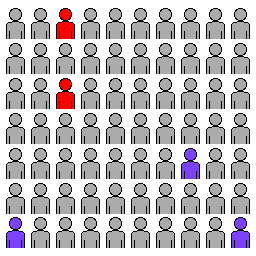
\includegraphics[width=0.15\textwidth]{figures/newEntity2}
\end{center}


}

%....................................................................................
%
%	Block
%
\block[titleleft,roundedcorners=16]{Graphical Record Linkage}{
	\raggedright

\setcounter{figure}{1}
\begin{center}
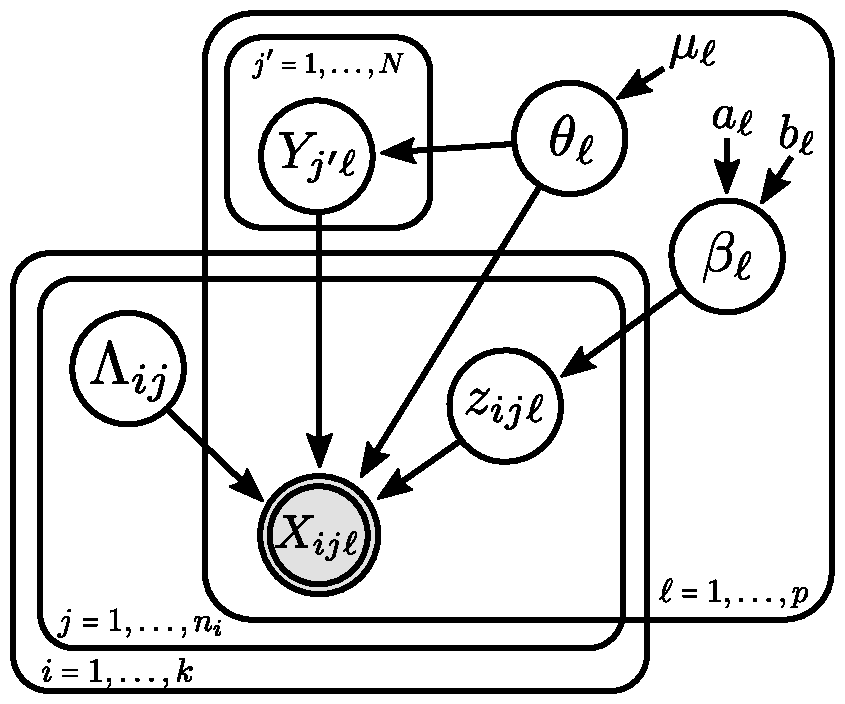
\includegraphics[width=0.25\textwidth]{figures/recordLinkage_graphicalModel}
%\caption{Graphical representation of models in \cite{steorts14smered, steorts15entity}.}
\end{center}

}

%....................................................................................
%
%	Block
%
\block[titleleft,roundedcorners=16]{Kullback-Leibler (KL) divergence}{


For any two distributions $P$ and $Q$, the maximum power for testing $P$ versus $Q$ is $$\exp\{-n D_{\text{KL}}(P || Q)\}.$$ 

\begin{itemize}
\item A low value of $D_{KL}$ means that we need many samples to distinguish $P$ from $Q.$

\item How  does changing $\bY$ (latent entity) or $\lam$ (linkage structure) change the distribution of $\bX$ (observed records)? 

\item We search for both meaningful upper and lower bounds. 
%\item Moreover, we investigate how well can we recover $\bY$ (latent entity) and $\lam$ (linkage structure) from $\bX$ (data).

\end{itemize}

\vspace*{1em}

Assuming the conditions of \cite{steorts14smered, steorts15entity}, 
let $$\mathcal{P} = \left\{f(X\mid \bY, \Lambda_{ij}, \bm{\theta}, \bm{\beta}): 
 \forall \Lambda_{ij} \in \{ 1, \ldots, N \}.\right\}$$
% Given $P, Q \in \mathcal{P}$, 

\begin{itemize}
\item  $X_1,X_2,\ldots,X_N$ are all independent given $(\bY,\lam, \bm{\theta}, \bm{\beta})$ under both $P, Q \in \mathcal{P}.$ 
\item This implies that  $D_{X_1, X_2, \ldots, X_N} (P \| Q) = \sum_i D_{X_i}(P \| Q).$
\end{itemize} 

	


	}
	




		
	
	
%..............................................................................................................................................................................................
%
%	CENTER COLUMN
%
\column{0.34}
%....................................................................................
%
% 	Block
%
\block[titleleft,roundedcorners=16]{Performance Bounds}{
	\raggedright
	

\begin{theorem}
\label{theorem:cat}
This result finds an upper bound on the KL divergence and a
 lower bound for the  probability that the categorical model in \cite{steorts14smered} gets the linkage structure incorrect. 
Let
$$\gamma = \max_{\Lambda_{ij} \neq \Lambda'_{ij}}
2\sum_{ij\ell} I(Y_{\Lambda_{ij}\ell} \neq Y_{\Lambda'_{ij}\ell}) (1-\beta_{\ell}) \ln \left \{
\dfrac{1}{
\min_m \theta_{\ell m} \beta_{\ell}} \right\}.$$
%
 \begin{enumerate}
\item[i)] The KL divergence is bounded above by $\gamma.$ That is,
$D_X(P || Q) \leq \gamma \enskip \forall P, Q \in \mathcal{P}$.
\item[ii)] The minimum probability of getting a latent entity wrong is
$Pr( {\Lambda}_{ij} \ne \Lambda^\prime_{ij}) \geq 1 - \dfrac{ \gamma + \ln 2}{\ln r}, \enskip \forall i,j$
\end{enumerate}
\end{theorem}
That is, as the latent entities become more distinct, $\gamma$ increases. On the other hand, as the latent entities become more similar, $\gamma \rightarrow 0.$ \\
\textbf{Remark}:
Consider Theorem \ref{theorem:cat} (i). Suppose $\beta_{\ell} \rightarrow 1.$ Then $D_{\bX} \geq 0.$ If instead $\beta_{\ell} \rightarrow 0,$ then $D_{\bX} \geq 1.$ The lower bound is only informative when $\beta_{\ell} \rightarrow 0.$ We have more information when the latent entities are separated.

\vspace*{2em}

\begin{theorem}
\label{theorem:string}
Assume string and categorical data $\bX$ as in \cite{steorts15entity} and distributions $P,Q \in \mathcal{P}$.  Assume two distinct linkage structures, denoted by $Y_{\Lambda_{ij}\ell}, Y_{\Lambda^\prime_{ij}\ell}.$
\begin{enumerate}
\item [i)] There is an upper bound on the KL divergence between any $P,Q \in \mathcal{P}$ 
given by $\kappa,$ that is $D_X(P||Q) \leq \kappa.$
%\begin{align}
%&D_{\bX}(P || Q)\\
% &\geq
%\sum_{i,j,\ell} 2(1 - \beta_\ell) \\
%& + \sum_{i,j,\ell}
%I(Y_{\Lambda_{ij}\ell} \neq Y_{\Lambda^\prime_{ij}\ell})
%\left(
%1 - e^{-c d(Y_{\Lambda_{ij}\ell}, Y_{\Lambda^\prime_{ij}\ell})}
%\right) E[ e^{-c  d(m, Y_{\Lambda_{ij}\ell})} ],
%\end{align}
\item [ii)] $Pr(\Lambda_{ij} \neq \Lambda^\prime_{ij}) \geq 1- \dfrac{\kappa + \ln 2}{\ln r},$
where 
\begin{align*}
\kappa &= \max_{\Lambda_{ij} \neq \Lambda^\prime_{ij}}\bigg[
2 \sum_{\ell} (1-\beta_\ell) I(Y_{\Lambda_{ij}\ell} \neq Y_{\Lambda^\prime_{ij}\ell}) 
  +  \\
& \qquad \sum_{\ell m}  I(Y_{\Lambda_{ij}\ell} \neq Y_{\Lambda^\prime_{ij}\ell}) 
 \left(
1 - e^{-c d(Y_{\Lambda_{ij}\ell}, Y_{\Lambda^\prime_{ij}\ell})}
\right) \\
&\times E[ e^{-c  d(m, Y_{\Lambda_{ij}\ell})} ] \bigg]\ln\{ (\min Q)^{-1} \}
\end{align*}
and $r+1$ is the cardinality of $\mathcal{P}$.
% where the expectation is taken according to 
%random variable $M \sim \alpha_\ell.$ That is, $\sum_m  \alpha_\ell (m)
%e^{-c  d(m, m^\prime)} $ is the moment generating function of $d(M,m^\prime)$ (evaluated at c).
\end{enumerate}
\end{theorem}


	
 }
%....................................................................................
%
%	Block
%
\block[titleleft,roundedcorners=16]{Priors on the Linkage Structure}{
	\raggedright
	\begin{itemize}
\item Above we a specific discrete uniform prior on $\lam$.  
\item We extend this to include other discrete uniform priors on $\lam$ including those that are informative. 
\item Special cases include the work of \cite{zanella2016microclustering, liseo_2011, sadinle_2014, pitman}. 
\item The theorem on performance bounds generalizes naturally, allowing comparisons to be made in future work. 
\end{itemize}
}
%..............................................................................................................................................................................................
%
% 	RIGHT COLUMN
%
\column{0.33}
%%....................................................................................
%
%	Block
%
\block[titleleft,roundedcorners=16]{Experiments}{
	\raggedright
	
In our experiments (\textbf{Experiment I} and \textbf{Experiment II}), synthetic categorical data are generated according to the 
Steorts, Hall Fienberg (2014, 2016) or Steorts (2015)  using the parameters in the figures below. 
\vspace*{1em} 

%\begin{itemize}
%\item In order to consider a realistic set of strings for $S$, we consider the set of 20 most popular female baby names from 2014, according to the United States Census. Then for the distance $d$, we consider the generalized Levenshtein edit distance.
%\item For each experiment, we vary exactly one of the parameters to demonstrate its impact of the linkage error rate $Pr( (\hat{\Lambda}_{ij}, \bY) \ne (\Lambda_{ij}, \bY))$. 
%\item We choose the other values such that the performance is neither extremely low nor extremely high. We set the distortion parameter $\beta_\ell$ to the same value for each $\ell$, i.e.\ $\beta_\ell = 0.6$ denotes a distortion probability of 0.6 for every field. $\beta_\ell = $ 0.0 to 1.0 means we started with $\beta_\ell = 0$ for all $\ell$ and swept the values until $\beta_\ell = 1$ for all $\ell$. \item Recall $p$ is the number of fields, and thus the maximum value of $\ell$. 
%\item We also set each $\theta_{\ell m}$ to the same value, i.e.\ $\theta_{\ell m} = 0.1$ denotes $\theta_{\ell m} = 0.1$ for all $\ell$ and all $m$. This further implies each field $\ell$ takes on exactly $M_\ell = 1/\theta_{\ell m}$ values in order for $\theta_\ell$ to be a valid probability distribution.
%\end{itemize}

\vspace*{1em} 

%\textbf{Categorical Experiments}:
%\begin{center}
%  \begin{tabular}{ l c c c c}
%    Experiment & $N$ & $\beta_\ell $ & $p = p_c$  & $\theta_{\ell m}$ \\ \hline
%    Fig. 1(a) & 10 to 500 & 0.6 & 3 & 0.1 \\
%    Fig. 1(b) & 100  & 0 to 1 & 3 & 0.1 \\
%    Fig. 1(c) & 100  & 0.6 & 1 to 8& 0.25 \\
%    Fig. 1(d) & 100  & 0.8  & 5& $\frac{1}{46} \text{ to } 1$
%  \end{tabular}
%%  \mycaption{Categorical Experiments}
%  \label{table:params}
%\end{center}
%
%\textbf{String Experiments}:
%\begin{center}
%  \begin{tabular}{ l c c c c c}
%    Experiment & $N$ & $\beta_\ell $ & $p = p_s$ & $c$ \\ \hline
%    Fig. 2(a) & 100 to 500 & 0.6  & 1 &  1.0 \\
%    Fig. 2(b) & 100  & 0.2 to 1 & 1  & 1.0 \\
%    Fig. 2(c) & 100  & 0.6 & 1 to 10  & 1.0 \\
%    Fig. 2(d) & 100  & 0.6 & 1 & 0 to 2
%  \end{tabular}
%%  \mycaption{String Experiments}
%  \label{table:params-str}
%\end{center}


\begin{center}
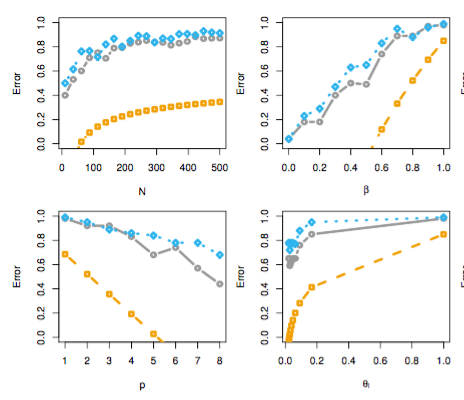
\includegraphics[width=0.25\textwidth]{figures/e1} \label{fig:cat}
%\mycaption{Theorem 1 (gold squares) holds on simulated
%    categorical records compared to exact sampling (grey circles) and Gibbs sampler (blue diamonds).}
\end{center}

\vspace*{1em} 

\begin{center}
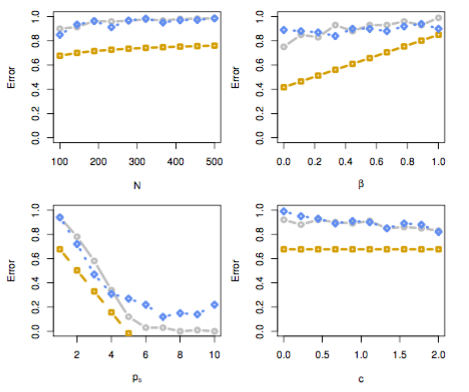
\includegraphics[width=0.25\textwidth]{figures/e2} \label{fig:str}
%\mycaption{Theorem 2 (gold squares) holds on simulated
%    noisy string records  compared to exact sampling (grey circles) and Gibbs sampler (blue diamonds).}
\end{center}






	
	}
%....................................................................................
%
%	Block
%
\block[titleleft,roundedcorners=16]{Conclusions and Acknowledgements}{
	\raggedright
	
\begin{itemize}
\item We have proposed the first performance bounds, to our knowledge, for record linkage models. 
\item Is it possible to prove tighter bounds?
\item Is it possible to compare to models outside of Gibbs partition prior models? 
%\item Can we avoid the label switching issue to make the performance bounds practical for real data?
\end{itemize}	

\vspace*{1em}

\textbf{Acknowledgements}: This work was supported in
part by NSF CAREER Award SES-1652431 and SES-1534412. This poster is based upon the original open source work of 
Sofia Jijon (https://sjijon.github.io). 
 }
\end{columns} 
%..............................................................................................................................................................................................
%
%	FOOT
%
%....................................................................................
%
%	References
%
\block[titleleft,roundedcorners=16]{}{
\small
\begin{minipage}{0.73\linewidth}
	\nocite{*}
	\bibliographystyle{unsrtnat}
	\bibliography{references}
 \end{minipage}
%....................................................................................
%
%	Logos
%
\begin{minipage}{0.2\linewidth}
\centering
	
\includegraphics[height=5cm]{Figures/Logo_GitHub}
\end{minipage}
}
%....................................................................................
%
%	My info
%
\note[width=14cm,targetoffsetx=3cm,targetoffsety=3cm,rotate=15]{
	\textbf{Contact information:}\\
	Rebecca C. Steorts\\
	resteorts.github.io
}
\end{document}